% ============================================================
% 高考模拟卷 LaTeX 模板
% 使用方法: 复制此模板,替换 {{科目}}, {{题量}}, {{总分}}, {{时间}} 等占位符
% 编译: xelatex -interaction=nonstopmode 文件名.tex
% ============================================================
\documentclass[12pt,a4paper]{article}
\usepackage[UTF8]{ctex}
\usepackage{geometry}
\usepackage{amsmath,amssymb,amsthm}
\usepackage{tikz,pgfplots}
\usepackage{enumitem}
\usepackage{tabularx}
\usepackage{fancyhdr}
\usepackage{graphicx}
\usepackage{xcolor}
\usepackage{ifthen}
% 化学需要: \usepackage[version=4]{mhchem}

\usetikzlibrary{calc,patterns,angles,quotes,arrows.meta,3d,positioning}
\pgfplotsset{compat=1.18}

\geometry{left=2.5cm,right=2.5cm,top=2.5cm,bottom=2.5cm}

\pagestyle{fancy}
\fancyhf{}
\fancyhead[C]{\small 2026年普通高等学校招生全国统一考试 {{科目}}}
\fancyfoot[C]{\thepage}
\renewcommand{\headrulewidth}{0.4pt}
\setlength{\headheight}{14pt}
\addtolength{\topmargin}{-2pt}

% 自动编号题目
\newcounter{question}
\newcommand{\question}[1][]{\refstepcounter{question}\par\noindent\textbf{\thequestion.}\ifthenelse{\equal{#1}{}}{}{~(#1分)}\quad}

\begin{document}

% ===== 封面 =====
\begin{center}
{\LARGE\bfseries 绝密★启用前}\\[0.5cm]
{\Huge\bfseries 2026年普通高等学校招生全国统一考试}\\[0.3cm]
{\Huge\bfseries (新高考I卷)}\\[0.5cm]  % 江苏卷改这里
{\Huge\bfseries {{科目}}}\\[0.8cm]
\end{center}

\noindent\textbf{本试卷共{{题量}}小题,满分{{总分}}分,考试时间{{时间}}分钟。}

\vspace{0.3cm}
\noindent\textbf{注意事项:}
\begin{enumerate}[leftmargin=2em]
\item 答卷前,考生务必将自己的姓名、准考证号填写在答题卡上。
\item 回答选择题时,选出每小题答案后,用铅笔把答题卡上对应题目的答案标号涂黑。如需改动,用橡皮擦干净后,再选涂其他答案标号。回答非选择题时,将答案写在答题卡上。写在本试卷上无效。
\item 考试结束后,将本试卷和答题卡一并交回。
\end{enumerate}

\vspace{0.5cm}
\hrule
\vspace{0.5cm}

% ===== 选择题模板 =====
\section*{一、选择题:...}

\setcounter{question}{0}

% --- 每道题的格式 ---
% 注释行写答案和思路,方便验证
% {{答案X}}
\question 题目内容(\quad)

% 选项横排(4列)
\begin{minipage}[t]{0.22\textwidth}A.~选项A\end{minipage}
\begin{minipage}[t]{0.22\textwidth}B.~选项B\end{minipage}
\begin{minipage}[t]{0.22\textwidth}C.~选项C\end{minipage}
\begin{minipage}[t]{0.22\textwidth}D.~选项D\end{minipage}

\vspace{0.5cm}

% --- TikZ图形示例 ---
% 函数图像
\begin{center}
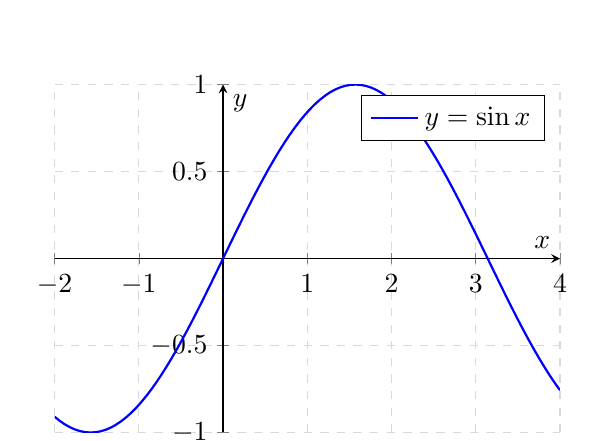
\begin{tikzpicture}
\begin{axis}[
    width=8cm,height=6cm,
    xlabel=$x$, ylabel=$y$,
    axis lines=middle,
    grid=major, grid style={dashed,gray!30},
    domain=-2:4, samples=100,
    legend pos=north east
]
\addplot[blue,thick] {sin(deg(x))};
\addlegendentry{$y=\sin x$}
\end{axis}
\end{tikzpicture}
\end{center}

% 几何图形
\begin{center}
\begin{tikzpicture}[scale=1.2]
\coordinate (A) at (0,0);
\coordinate (B) at (4,0);
\coordinate (C) at (1.5,3);
\draw[thick] (A)--(B)--(C)--cycle;
\node[below left] at (A) {$A$};
\node[below right] at (B) {$B$};
\node[above] at (C) {$C$};
\end{tikzpicture}
\end{center}

% 3D立体几何
\begin{center}
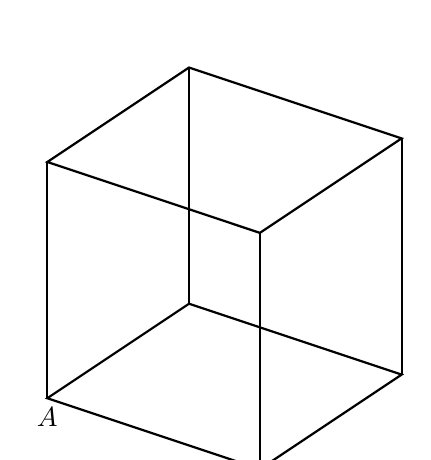
\begin{tikzpicture}[scale=1, x={(0.9cm,-0.3cm)}, y={(0.6cm,0.4cm)}, z={(0cm,1cm)}]
\coordinate (A) at (0,0,0); \coordinate (B) at (3,0,0);
\coordinate (C) at (3,3,0); \coordinate (D) at (0,3,0);
\coordinate (A1) at (0,0,3); \coordinate (B1) at (3,0,3);
\coordinate (C1) at (3,3,3); \coordinate (D1) at (0,3,3);
% 底面
\draw[thick] (A)--(B)--(C)--(D)--cycle;
% 顶面
\draw[thick] (A1)--(B1)--(C1)--(D1)--cycle;
% 侧棱
\draw[thick] (A)--(A1); \draw[thick] (B)--(B1);
\draw[thick] (C)--(C1); \draw[thick] (D)--(D1);
\node[below] at (A) {$A$};
\end{tikzpicture}
\end{center}

% ===== 解答题模板 =====
\section*{二、解答题:...}

\question[13] 解答题内容...

% ===== 结尾 =====
\end{document}
